IEEE $802.11$ networks use a shared and limited medium to establish communication among nodes. Carrier Sense Multiple Access with Collision Avoidance (CSMA/CA) is the protocol in charge of coordinating access to the wireless medium in order to avoid simultaneous transmissions by different nodes. If two or more nodes ($N$) attempt transmission at the same time, a \emph{collision} occurs and the resulting transmission is discarded by the receivers.

Carrier Sense Multiple Access with Enhanced Collision Avoidance (CSMA/ECA)~\cite{CSMA_ECA} was introduced as an enhancement to CSMA/CA. It is capable of achieving a collision-free state by making very simple changes on the way CSMA/CA behaves.

Performance evaluation for CSMA/ECA have been presented in~\cite{E2CA_performance}. Nevertheless, to the best of our knowledge this is the first work that introduces further enhancements to the protocol, making it possible to allocate a larger number of contenders and achieve greater throughput than CSMA/CA while providing the same service time to all users.

\section{Related work}

Time in WLANs is slotted, and each slot can be classified as empty, successful or collision (accounting for no transmission, successful transmission or collision, respectively).

In CSMA/CA, each contender attempting to transmit a packet chooses a uniformly random backoff counter value $B = [0,CW(k)-1]$, where $k=[0,\ldots,m]$ is the \emph{backoff stage} and $CW(k)=[2^{k}CW_{\min},~2^{m}CW_{\min}]$ is the contention window, with $CW_{\min}$ its minimum value. Each passing empty slot decrements $B$ by one; when the backoff counter reaches zero, the contender will attempt transmission. The success of the transmission attempt is only confirmed by the reception of an acknowledgement (ACK) frame from the receiver, otherwise a collision is assumed. If that is the case, each contender involved in the collision doubles its contention window by incrementing its backoff stage and the packet is retransmitted. If the transmission is successful, the sender resets its contention window to the minimum value ($k=0\therefore CW(k)=CW_{\min}$).

CSMA/ECA achieves less collisions and outperforms CSMA/CA in most typical scenarios~\cite{CSMA_ECA}. The only difference with CSMA/CA is that a deterministic backoff~$B=N_{\max}$ is chosen after each successful transmission. $N_{\max}$ is defined in~(\ref{eq:capacity}) as the \emph{collision-free constraint} and represents the maximum number of nodes participating in the contend for transmission able to achieve a collision-free state.

\begin{equation} \label{eq:capacity}	
	N_{\max} = CW_{\min}/2
\end{equation}

In a scenario where $N\leq N_{max}$, eventually all contenders will be able to pick different transmission slots, therefore achieving a collision-free state.

When the system is overcrowded, $N>N_{\max}$, CSMA/ECA suffers a decrease in throughput as seen in Figure~\ref{fig:throughput}. This effect is caused by collisions originated by $N-N_{\max}$ contenders forced to generate a random backoff counter and attempting transmission on slots previously picked by $N_{\max}$ nodes using a deterministic backoff.


\begin{figure}[htbp]
  \centering
  \includegraphics[width=0.7\linewidth, angle = -90]{figures/errorPlots/ECA-vs-CA-fixed.eps}
  \caption{The throughput is CSMA/ECA decreases when the number of contenderes~$N$~exceeds~$N_{\max}$, which is the maximum number of contenders that can be allocated in a collision-free fashion.
  \label{fig:throughput}}
\end{figure}

As $N-N_{\max}$ nodes are unable to successfully transmit, collisions force the $N_{\max}$ nodes that chose a deterministic backoff, to switch to a random one. The outcome is a mixed system composed of contenders using either deterministic or random backoff counters. The throughput degradation depicted in Figure~\ref{fig:throughput} when $N=16$, is a consequence of the great number of collisions resulting from this behavior.